\documentclass[polish,polish]{article}
\usepackage{amssymb}
\usepackage[a4paper, textheight=25cm]{geometry}
\usepackage{datetime}
\usepackage[margin=2em, font=small,labelfont=it]{caption}
\usepackage[T1]{fontenc}
\usepackage[utf8]{inputenc}
\usepackage{babel}
\usepackage{pslatex}
\usepackage{tikz}
\usepackage{latexsym}
\usepackage{graphicx}
\usepackage{mathpazo} % use palatino
\usepackage[scaled]{helvet} % helvetica
\usepackage{microtype}
\usepackage{amsmath}
\usepackage{subfigure}
\usepackage{hyperref}
\usepackage{blindtext}
\usepackage{float}
\usepackage{tabularx}
\usepackage{gensymb}
\usepackage{lscape}
% !!! do obracania
% sidewaysfigure, sidewaystable
\usepackage{rotating}
\usepackage{tikz}
\usepackage{xcolor}
\usepackage{listings}

\lstdefinestyle{Python}{
    language        = Python,
    basicstyle      = \ttfamily,
    commentstyle    = \color{green}\ttfamily,
    keywordstyle    = \color{blue},
    stringstyle     = \color{brown},
    otherkeywords={self,assert,True,False},
}

\DeclareUnicodeCharacter{23A1}{⎡}
\DeclareUnicodeCharacter{23A5}{⎢}
\DeclareUnicodeCharacter{23A3}{⎣}
\DeclareUnicodeCharacter{23A4}{⎤}
\DeclareUnicodeCharacter{23A2}{⎥}
\DeclareUnicodeCharacter{23A6}{⎦}
\DeclareUnicodeCharacter{207CE}{Θ}

% Letterspacing macros
\newcommand{\spacecaps}[1]{\textls[30]{\textbf{#1}}}
\newcommand{\spacesc}[1]{\textls[50]{\textsc{\MakeLowercase{#1}}}}

% przeciążenia poszczególnych referencji autoref
\def\figureautorefname{\emph{rys.}}
\def\sectionautorefname{\emph{rozdz.}}
\def\subsectionautorefname{\emph{rozdz.}}
\makeatletter
\newcommand*{\rom}[1]{\expandafter\@slowromancap\romannumeral #1@}
\makeatother
% przeciążenie domyślnych symboli w itemize
\renewcommand\labelitemi{--}

\begin{document}
\lstset{
    frame       = single,
    numbers     = left,
    showspaces  = false,
    showstringspaces    = false,
    captionpos  = t,
    caption     = \lstname,
    breaklines=true,
}
\begin{titlepage}
\newcommand{\HRule}{\rule{\linewidth}{0.5mm}} % Defines a new command for the horizontal lines, change thickness here

\center % Center everything on the page
 
%------------------------------------------------------------------
%	HEADING SECTIONS
%------------------------------------------------------------------

\textsc{\LARGE Politechnika Wrocławska}\\[0.25cm] % Name of your university/college
\textsc{\Large Wydział Elektroniki}\\[0.75cm] % Name of your university/college
\textsc{\Large Automatyka i Robotyka}\\[0.3cm] % Major heading such as course name
\textsc{\large Roboty Mobilne 2 -- Laboratorium}\\[0.5cm] % Minor heading such as course title

%------------------------------------------------------------------
%	TITLE SECTION
%------------------------------------------------------------------

\HRule \\[0.4cm]
{ \huge \bfseries Sterowanie kinematyczne 4-5 manipulatorów z uwzględnieniem interakcji z obiektem \\
\normalsize \Large Zakończenie }\\[0.4cm] % Title of your document
\HRule \\[1.5cm]
 
%------------------------------------------------------------------
%	AUTHOR SECTION
%------------------------------------------------------------------

\begin{minipage}{0.4\textwidth}
\begin{flushleft} \large
\emph{Autorzy:}\\
Jakub \textsc{Gabała}, \textit{230991}\\ % Your name
Maciej \textsc{Kajdak}, \textit{226256}\\ % Your name
\end{flushleft}
\end{minipage}
~
\begin{minipage}{0.4\textwidth}
\begin{flushright} \large
\emph{Opiekun:} \\
dr inż. Andrzej \textsc{Wołczowski} % Supervisor's Name
\end{flushright}
\end{minipage}\\[2cm]

%------------------------------------------------------------------
%	DATE SECTION
%------------------------------------------------------------------

{\large \today}\\[2cm] % Date, change the \today to a set date if you want to be precise
 
%------------------------------------------------------------------

\vfill % Fill the rest of the page with whitespace

\end{titlepage}

\section{Wstęp}
W temacie opracowywania sterowania kinematycznego dla protezy dłoni złożonej z kilku manipulatorów projekt pokierował się w stronę programistyczną. 
Opracowywane jest narzędzie, w którym wszystkie obliczenia potrzebne do opisywania kinematyki oraz sterowania takim układem, mogą być tworzone i obliczane w stosunkowo szybkim czasie dzięki zaimplementowaniu potrzebnego zaplecza matematycznego oraz teorii robotycznej. 
Do tej pory stworzone zostały:
\begin{itemize}
\item[$\checkmark$] Moduł obliczania kinematyki oraz transformacji pomiędzy układami w przestrzeni konfiguracyjnej manipulatora.
\item[$\checkmark$] Moduł zachowywania obliczonych elementów w celu ich późniejszego wykorzystania bez potrzeby ponownych obliczeń
\item[$\checkmark$] Stworzenie wizualizacji przestrzennej z wykorzystaniem narzędzia gnuplot
\end{itemize}


\newpage
\section{Wykorzystane oprogramowanie}

Wszystkie obliczenia prowadzone są dzięki wykorzystaniu języka Python. 
Jest to język skryptowy, niezwykle często uzywany do prototypowania programów albo prostych w implementacji obliczeń.

Obliczenia symboliczne, które wykonywane są dla poszczególnych macierzy, możliwe są dzięki wykorzystaniu pakietu \textbf{Sympy} dostępnym na zasadach wolnego oprogramowania na licencji BSD. Przykładowy kod z wykorzystaniem modułu Sympy przedstawiono na listingu \ref{lst:sympy}.

Aby możliwe było przenoszenie obliczonych rozwiązań oraz nie powtarzanie obliczeń użyto pakietu marshal umożliwiającego zapisywanie obliczeń oraz ponowne ich ładowanie. Obliczone wyrażenia zapisywane są w postaci pliku, więc zapewniona jest przenośność między systemami.

Wszystkie elementy są tworzone pod kątem obliczeń dla protezy dłoni przedstawionej w poprzednich pracach \cite{wolczowski2016control}



\begin{lstlisting}[caption={Przykład pracy w środowisku sympy},
     label={lst:sympy}
     ]
>>>theta = sym.symbols("Theta")
...R = sym.Matrix([[cos(theta), -sin(theta)	, 0, 0],
...                [sin(theta), cos(theta)	, 0, 0],
...                [0		  , 0		, 1, 0],
...                [0		  , 0		, 0, 1]])
>>>R
Matrix([
[cos(Theta), -sin(Theta), 0, 0],
[sin(Theta),  cos(Theta), 0, 0],
[         0,           0, 1, 0],
[         0,           0, 0, 1]])
>>>T=sym.Matrix([[1, 0, 0, 1],
              	 [0, 1, 0, 2],
              	 [0, 0, 1, 3],
              	 [0, 0, 0, 1]])
>>>R*T
Matrix([
[cos(Theta), -sin(Theta), 0, -2*sin(Theta) + cos(Theta)],
[sin(Theta),  cos(Theta), 0,  sin(Theta) + 2*cos(Theta)],
[         0,           0, 1,                          3],
[         0,           0, 0,                          1]])
\end{lstlisting}


\newpage
%------------------------------------------------------------------
\section{Środowisko pracy}
W wyniku prac nad narzędziem tworzonym w ramach projektu udało się zaimplementować potrzebne operacje wymagane przy obliczeniach roboycznych. Przykładowa funkcja obliczająca macierz transformacji na podstawie danych podawanych w notacji Denavita-Hartenberga została przedstawiona na listingu \ref{lst:transformation}. Funkcja używa również innych zadeklarowanych funkcji, czyli funkcji obliczających macierz rotacji oraz translacji (druga przedstawiona na listingu \ref{lst:translation}).

\begin{lstlisting}[style = Python,
     caption={Funkcja obliczająca macierz transformacji},
     label={lst:transformation}
   ]
def m_transformation(Rz, Tz, Tx, Rx, use_degrees=True, simplify=True):
    """
    Defines a transformation in Denavit-Hartenberg notation.

    :param Rz: variable used in z-rotation matrix
    :param Tz: variable used in z-translation matrix
    :param Tx: variable used in x-translation matrix
    :param Rx: variable used in x-rotation matrix
    :param use_degrees: uses degrees if True, uses rads otherwise
    :param simplify: simplifies expression if True, does not simplify otherwise
    :type Rz: numbers.Number or sympy.Symbol
    :type Tz: numbers.Number or sympy.Symbol
    :type Tx: numbers.Number or sympy.Symbol
    :type Rx: numbers.Number or sympy.Symbol
    :type use_degrees: bool
    :type simplify: bool
    :return: evaluated matrix
    :rtype: object inheriting from sym.matrices.MatrixBase
    """
    K = m_rot('z', Rz, use_degrees) * m_trans('z', Tz) * m_trans('x', Tx) * m_rot('x', Rx, use_degrees)
    if simplify:
        K = sym.simplify(K)
    return K
\end{lstlisting}

Rozbudowując środowisko uzyskujemy narzędzie do obliczeń robotycznych dla manipulatorów. 
Wszystkie parametry podawane są do odpowiednich funkcji a zwracane przezeń obiekty mogą zostać zapisane do pliku, dzięki czemu ponowne ich obliczanie nie jest potrzebne i w ten sposób oszczędzany jest czas na obliczenia, które, co należy zaznaczyć, mają stosunkowo duży nakład czasowy, szczególnie w przypadku algorytmu kinematyki odwrotnej.

\newpage
\begin{lstlisting}[style = Python,
     caption={Funkcja obliczająca macierz translacji},
     label={lst:translation}
   ]
def m_trans(axis, variable):
    """
    Defines a translation matrix in Denavit-Hartenberg notation.

    :param axis: one of Cartesian coordinate system axes (x, y, z)
    :param variable: variable defining translation
    :type axis: char
    :type variable: numbers.Number or sympy.Symbol
    :return: evaluated matrix
    :rtype: object inheriting from sym.matrices.MatrixBase
    """

    # check if axis provided is correct
    ax = axis.lower()
    assert ax in ['x', 'y', 'z'], "Invalid axis provided."

    # checks if variable is a Symbol or a number
    assert len([t for t in [numbers.Number, sym.Symbol, sym.Mul] if
                isinstance(variable, t)]) == 1, "'variable' should be a sympy.Symbol, a number or an expression."

    var = variable

    return sym.N(sym.Matrix([
        [1, 0, 0, {'x': var}.get(ax, 0)],
        [0, 1, 0, {'y': var}.get(ax, 0)],
        [0, 0, 1, {'z': var}.get(ax, 0)],
        [0, 0, 0, 1, ]
    ]), 5, chop=True)
\end{lstlisting}

Dzięki takim operacjom możliwe jest zaimplementowanie algorytmu bazującego na transformacjach pomiędzy układami w obie strony.

Algorytm Newtona implementowany w stworzonym narzędziu bazuje na iteracyjnym podejściu do zadania sterowania, co zostało opisane wcześniej \cite{kumar2015inverse}. 
Oblicza na podstawie odwrotnej kinematyki konfigurację manipulatora dla ustalonego kroku pomiędzy stanami i w ten sposób tworzy trajektorię, po której porusza się każdy przegub traktowany jako osobny manipulator. 
W algorytmie ważny jest też dopuszczalny błąd oraz maksymalna ilość iteracji przy rozwiązywaniu problemu.
W każdej iteracji sprawdzany jest obecny błąd czyli różnica pomiędzy celem a obecną koordynacją (ta różnica obliczana jest na podstawie długości wektora rozłożonego pomiędzy oboma punktami w przestrzeni).
W wypadku, gdyby przekroczono ilość możliwych iteracji zwracana jest stworzona -- niekompletna trajektoria.
Iteracyjna postać algorytmu przedstawia się równaniem \ref{eq:newton}.

\begin{equation}
f(q) = f(q_{0}) + \frac{\partial f}{\partial q}(q_{0})(q - q_{0})
\label{eq:newton}
\end{equation}

\newpage
\section{Wizualizacja}

Przy użyciu narzędzia gnuplot dostępnego na zasadzie wolnego oprogramowania zrealizowano prostą wizualizację 3D sterowanej dłoni.
Przykład działania pokazano na rysunkach \ref{fig:proteza} oraz \ref{fig:proteza2}.
Dzięki takiemu narzędziu łatwiej analizować i testować wyniki, jakie daje tworzone narzędzie do obliczeń robotycznych.

\begin{figure}[H]
\centering
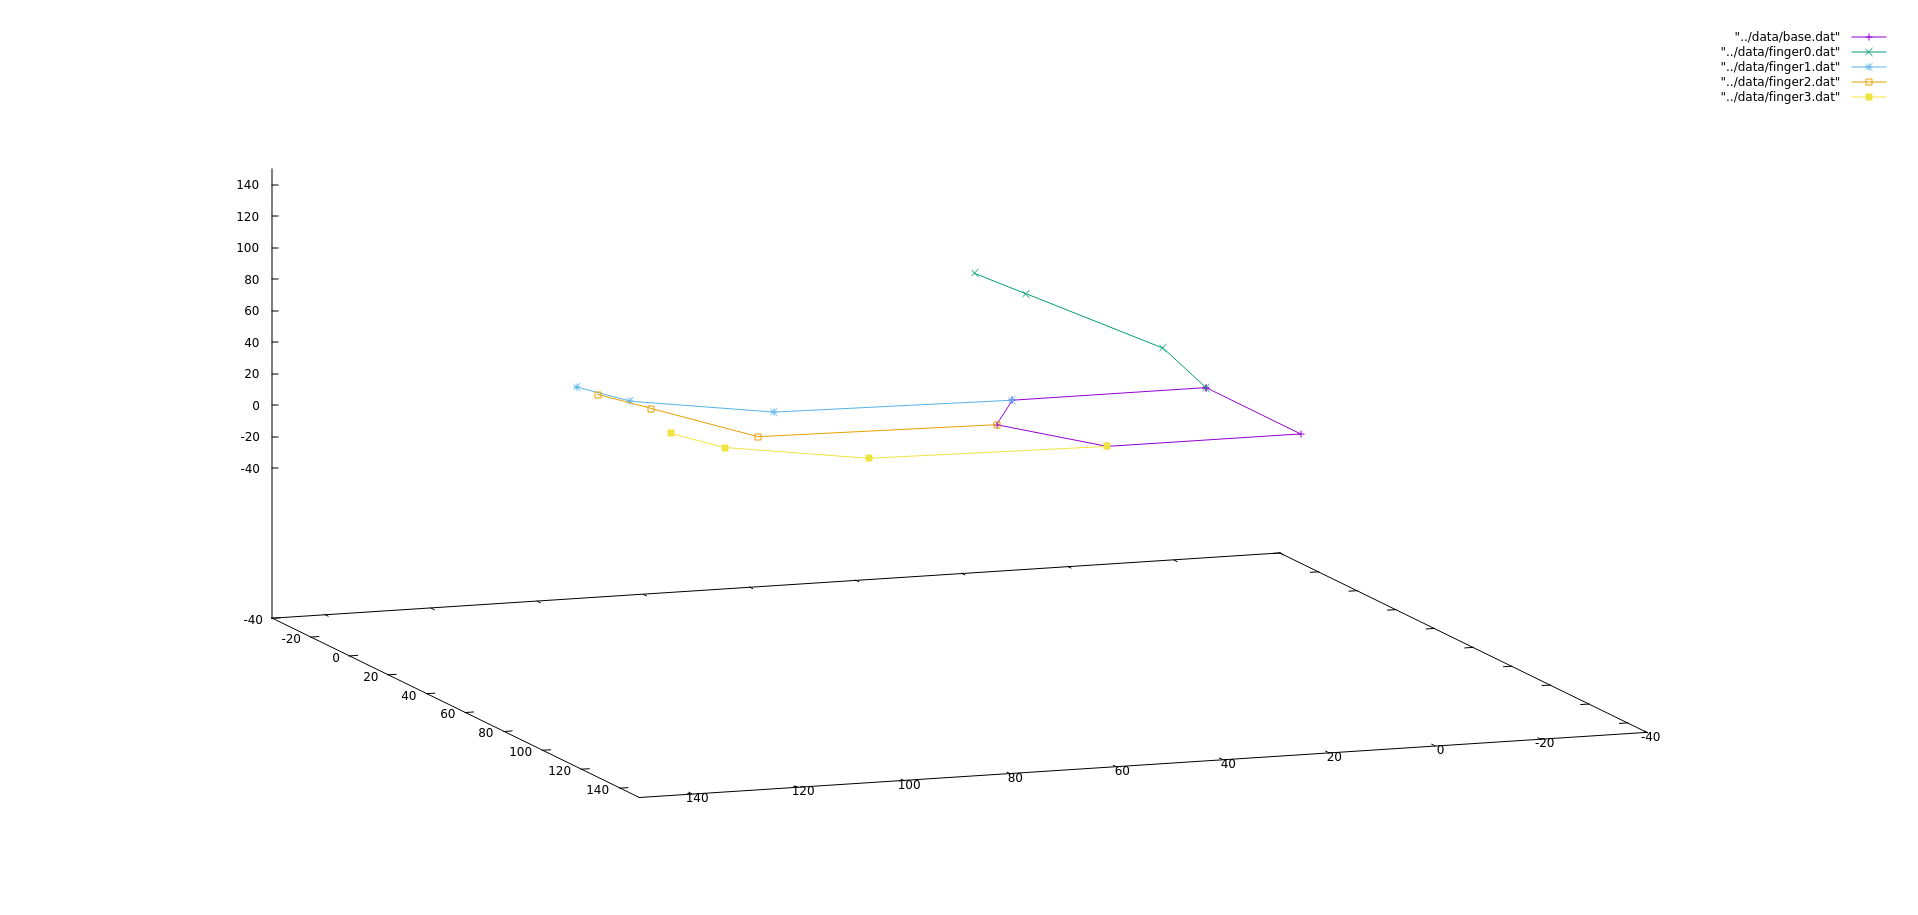
\includegraphics[width=.7\textwidth]{plot.png} 
\caption{Przykład działania wizualizacji robotycznej protezy dłoni}
\label{fig:proteza}
\end{figure}

\begin{figure}[H]
\centering
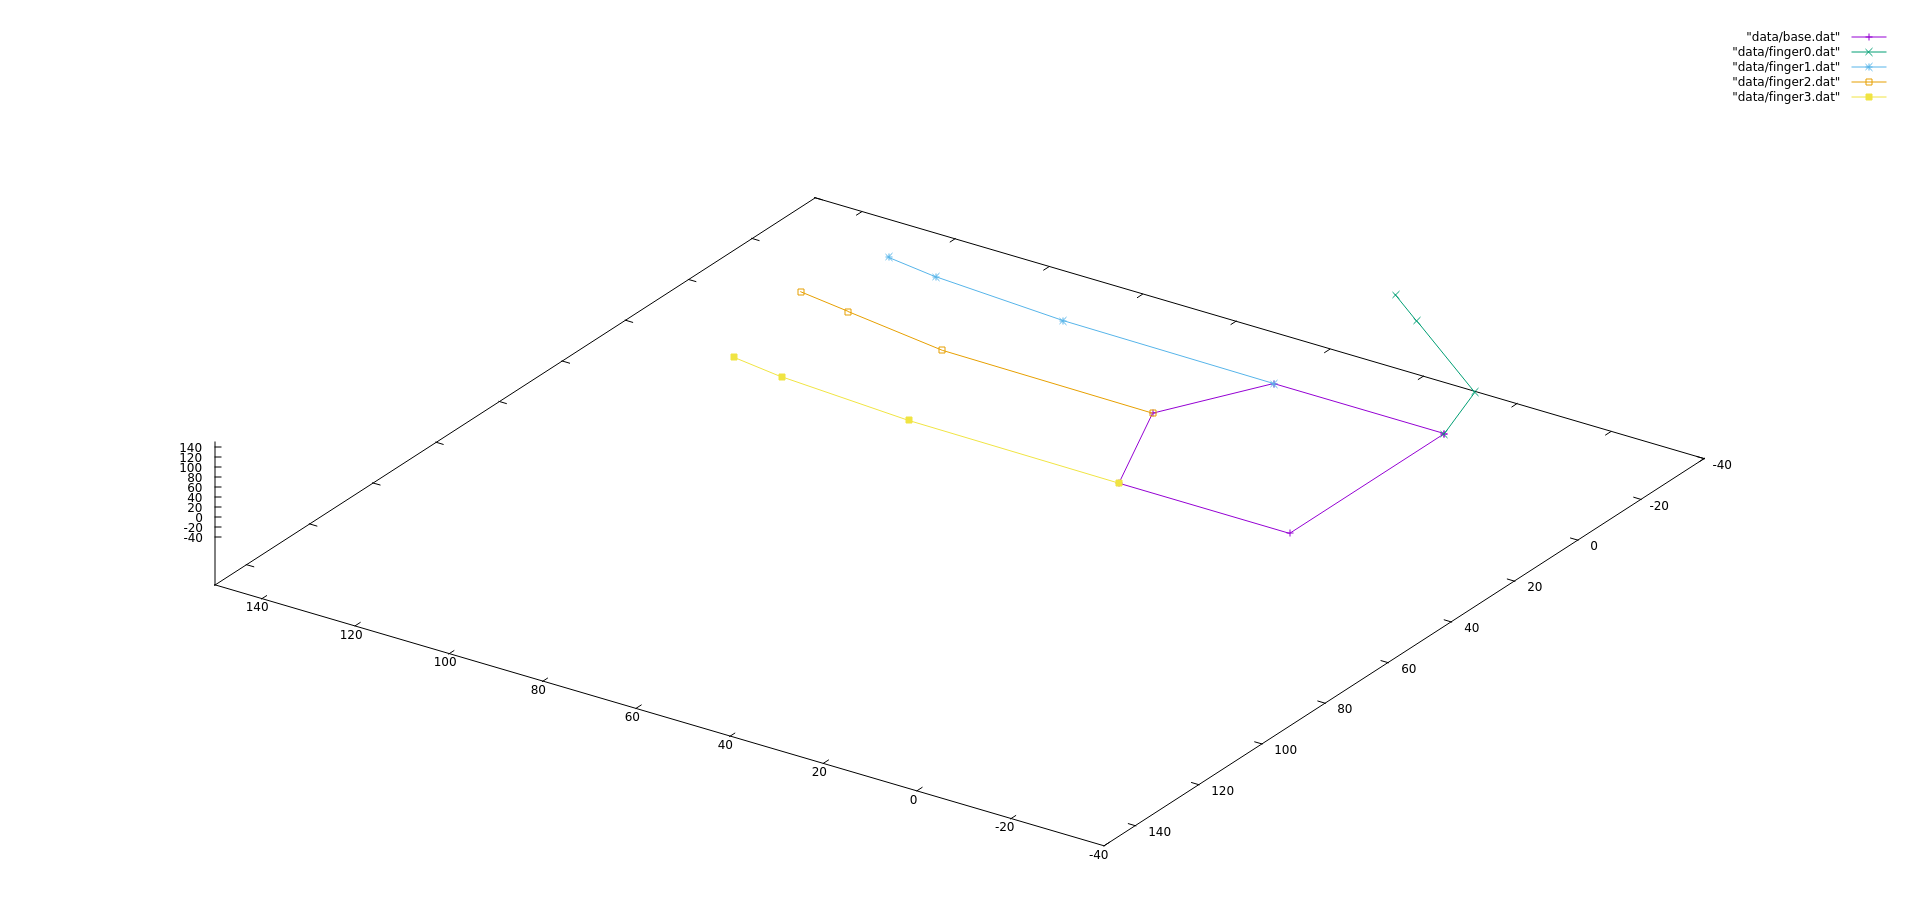
\includegraphics[width=.7\textwidth]{plot2.png} 
\caption{Przykład działania wizualizacji robotycznej protezy dłoni}
\label{fig:proteza2}
\end{figure}

Cały kod programów oraz dokumentacja całej biblioteki do obliczeń robotycznych znajduje się pod adresem internetowym \url{https://github.com/jjmgab/RM2_hand-control} w repozytorium autorów.

\newpage
\bibliographystyle{plabbrv} 
\bibliography{bibliografia}


\end{document}